\chapter{Experiments}

\section{Datasets}
\label{sec:exp-datasets}

\subsection{MPII Human Pose}
\label{sec:exp-mpii}

In \cite{andriluka_2d_2014}, the authors present a dataset for 2D human pose estimation on still images.
It contains $25.000$ images, where $40.000$ persons were annotated.
The annotations include $16$ joint annotations in addition to an indicator of whether or not the joint is visible or not.
The $16$ joints are \textit{left / right ankle}, \textit{left / right knee}, \textit{left / right hip}, \textit{left / right elbow}, \textit{left / right shoulder}, \textit{left / right wrist}, \textit{pelvis}, \textit{thorax}, \textit{upper neck} and \textit{top of the head}.
See \fref{fig:mpii_example_images} for example images of the dataset.
In addition, the body center coordinates are given in addition to a scale indicating the size of the person bounding box w.r.t. $200$ pixels.
Also, a bounding box of the head is given, which is used to compute the \textit{PCKh} metric (see \sref{sec:exp-pckh}).
The images were extracted from YouTube videos and do not contain artifacts commonly found in videos like compression or blur.
Additionally, each image is assigned an activity performed in the video it was extracted from, totalling $401$ total activities.
However, these annotations were not used for Human Action Recognition since they are too fine-grained and the number of samples per activity is too low for training a deep neural network.

\begin{figure}[htb!]
    \centering
    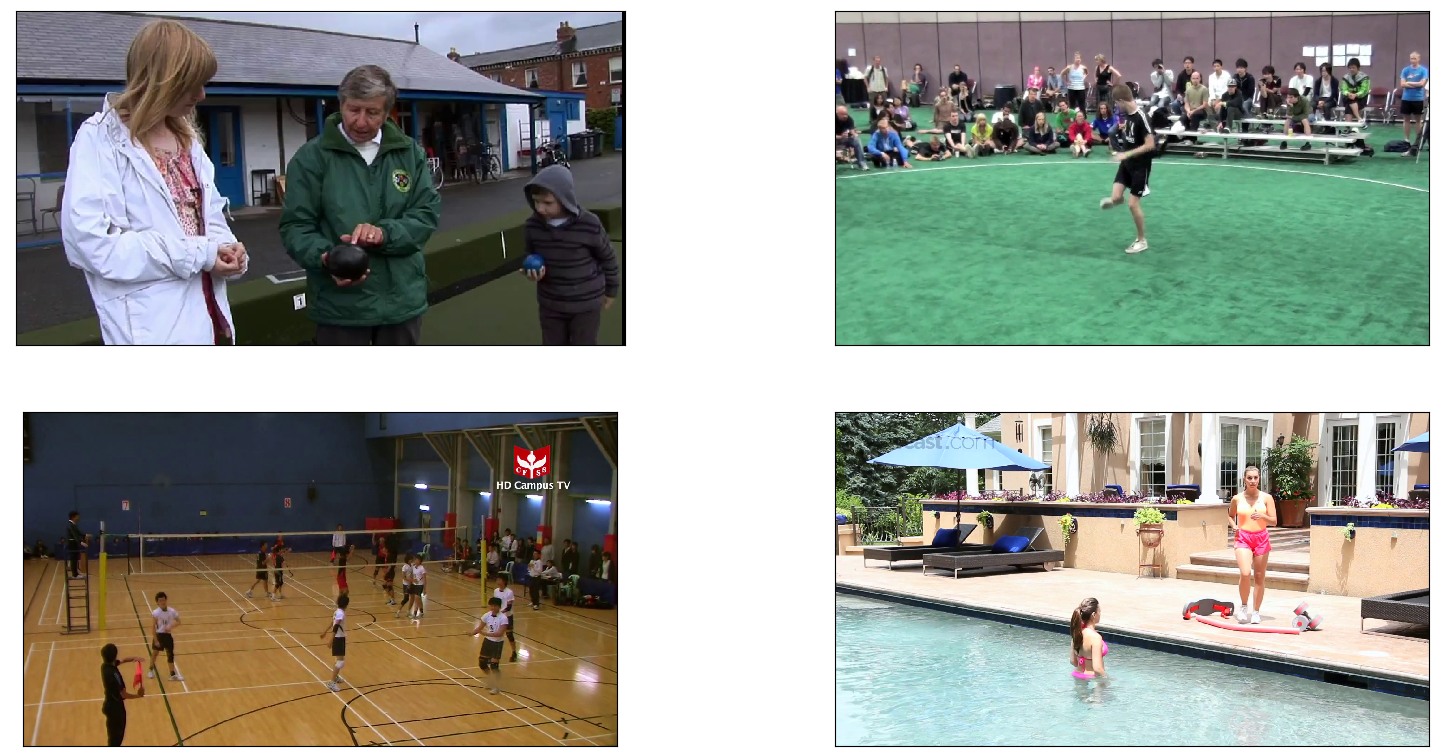
\includegraphics[width=0.7\textwidth]{mpii_example_images.png}
    \caption{Four example images from the MPII dataset \cite{andriluka_2d_2014}. }
    \label{fig:mpii_example_images}
\end{figure}

We follow the approaches from \cite{luvizon_2d/3d_2018} for preprocessing, which the authors present in their supplemental material.
First, a person bounding box is estimated using the center body annotation from the dataset.
The authors multiply the scale given by the annotation $s_{orig}$ by $1.25$, resulting in $s_{new}$.
They do not motivate the reason for using this specific value, but it most likely was used to enlarge the bounding box to contain more context around the person.
Next, they compute the width and height using $s_{new} \cdot 200$, which results in a square bounding box.
In addition, the authors also alter the center position $(c_x,  c_y)$ given by the annotation by computing $(c_{x}^{new}, c_y^{new}) = (c_x, c_y + s_{new} \cdot 12)$.
Again, the authors do not provide a reasoning for moving the center position further towards the neck of the person in this way.
Once the bounding box is computed, the image is cropped to the size of the bounding box around the newly computed center coordinate and rescalled to a size of $256 \times 256$ .
In the case where a joint annotation falls outside of the now cropped image, the authors set the visibility of the joint to $0$ and set the $(x,y)$ coordinates of the joint to $(-1e9, -1e9)$.

Additionally, the authors introduce parameters used for augmentation.
These values are sampled from their respective sets whenever augmentation is performed.
Specifically, they introduce $s_{aug} \in \{0.7, 1, 1.3\}$ which gets multiplied with $s_{new}$ computed earlier.
Also, $r_{aug} \in \{-40, -35, \dots, 35, 40\}$ is introduced to rotate the image $r_{aug}$ degrees around its center, possibly introducing black borders around the image.
Moreover, when augmenting, the image is horizontally flipped with a chance of $50$ percent.
See \fref{fig:mpii_example_augmentation} for multiple examples of different augmented images, including augmented pose. 

\begin{figure}[htb!]
    \centering
    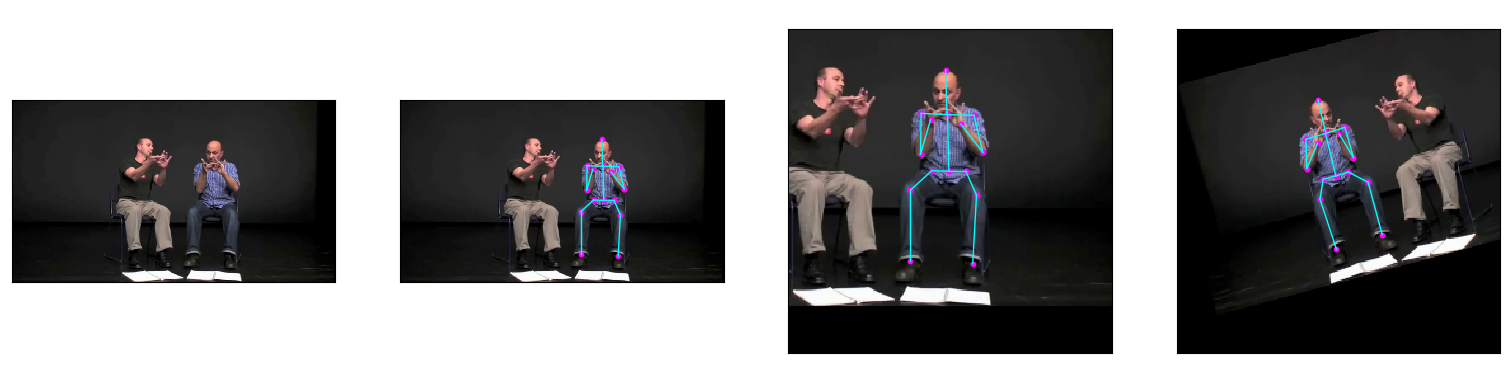
\includegraphics[width=0.99\textwidth]{mpii_dataset_augmented_examples.png}
    \caption{\textbf{From left to right}: \textbf{1.} Original image from the MPII dataset. \textbf{2.} Original image with the ground truth pose superimposed. \textbf{3.} Image after estimating the bounding box, cropping and rescaling. \textbf{4.} Augmented image using $s_{aug} = 1.3$, $r_{aug} = -15$ degrees and flipping the image vertically.}
    \label{fig:mpii_example_augmentation}
\end{figure}


The dataset does not contain annotations for the test data, other than the scale and center coordinates.
To evaluate the test images, the joints need to be evaluated and the results need to be send to the authors for comparison to the ground truth pose.
This ensures that the test data annotations are not mistakenly or maliciously used in training.
For all datasets used in the experiments, $10$ percent of the training datapoints were withheld from training and used as validation data.

\subsection{Penn Action}
\label{sec:exp-penn}

Another dataset used in \cite{luvizon_2d/3d_2018} is the Penn Action dataset \cite{zhang_actemes_2013}.
It contains $2326$ video clips of $15$ different actions performed.
The actions performed are mostly sports related and include \textit{baseball swing}, \textit{clean and jerk}, \textit{jumping jacks}, \textit{pushup}, \textit{strum guitar}, \textit{bench press}, \textit{golf swing}, \textit{baseball pitch}, \textit{situp}, \textit{tennis forehand}, \textit{bowling}, \textit{jump rope}, \textit{pullup}, \textit{squat} and \textit{tennis serve}.
In addition, the authors provide annotations for $13$ body joints,
including \textit{left and right shoulders, elbows, wrists, hips and knees} as well as one annotation of the \textit{head} of the person.
Some example images can be seen in \fref{fig:pennaction_example_images}. 

\begin{figure}[htb!]
    \centering
    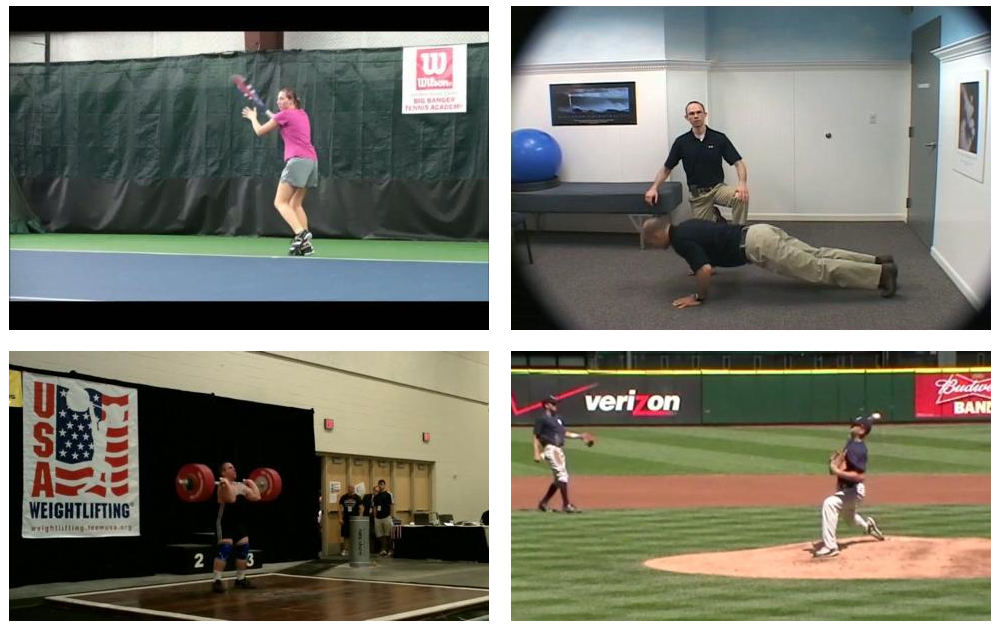
\includegraphics[width=0.7\textwidth]{pennaction_example_images.png}
    \caption{Four example images from the Penn Action dataset \cite{zhang_actemes_2013}. }
    \label{fig:pennaction_example_images}
\end{figure}

It was decided by \cite{luvizon_2d/3d_2018} that the number of joints should be identical to the ones presented in \cite{andriluka_2d_2014} \sref{sec:exp-mpii} because the network assumes a fixed number of joints.
This then means that the network architecture does not need to be changed, no matter which dataset is used.
Specifically, the \textit{pose cube} dimensionality does not need to be changed.
To achieve this, the \textit{head} annotation of the Penn Action dataset is mapped to the \textit{upper neck} joint of the MPII dataset and the missing joints were interpreted as not visible.
The augmentation is identical to the augmentation mentioned in \sref{sec:exp-mpii}.

For some experiments, we compute a ground truth bounding box of the person by calculating the minimum and maximum $x$ and $y$ coordinates of the pose and defining these as the corners of the bounding box.
Additionally, to include more context, we decided to increase the bounding box by $30$ pixels in both dimensions.

Additionally, the authors in \cite{luvizon_2d/3d_2018} decide to process the video clips in chunks of $16$ frames.
This is again important since the network architecture can be kept the same because \textit{pose cube} dimensions do not change that way.
Thus, we decided to precompute $16$ frames subclips, which we call \textit{fragments}, and save them separately to increase the training speed, since the preprocessing and extraction of the subclips does not need to be done at training time. 

\subsection{JHMDB}
\label{sec:exp-jhmdb}

Similar to \cite{zhang_actemes_2013} \sref{sec:exp-penn}, the JHMDB dataset \cite{jhuang_towards_2013} contains annotations for pose and action in video clips.
The dataset was created by taking a subset of the HMDB action recogntion dataset \cite{kuehne_hmdb:_2011}, which was then annotated using the \textit{puppet tool} \cite{zuffi_pictorial_2012}.
This tool allows to not only annotate the pose of the person but also automatically computes a binary segmentation map of the person, further referred to as the \textit{puppet mask}.
See \fref{fig:puppet_tool_example} for a visualization of the annotation process and the puppet tool.

\begin{figure}[htb!]
    \centering
    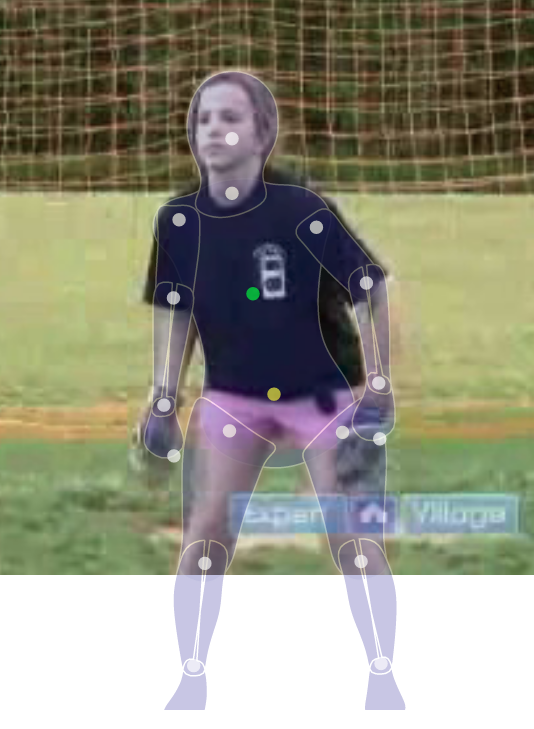
\includegraphics[width=0.4\textwidth]{puppet_tool_example.png}
    \caption{Example of an image, annotated using the puppet flow. The dots indicate the joint positions, while the transparent human figure prior automatically adjusts, yielding the human segmentation map. Notice that, by using the figure, even joints that are not visible (like the ankles) still get anatomically plausible annotations. Image taken from \cite{noauthor_jhmdb_nodate}.}
    \label{fig:puppet_tool_example}
\end{figure}

The clips in the HMDB dataset were taken from YouTube.
The annotated subset contains the following actions:
\textit{brush hair}, \textit{catch}, \textit{clap}, \textit{climb stair}, \textit{golf}, \textit{jump}, \textit{kick ball}, \textit{pick}, \textit{pour}, \textit{pullup}, \textit{push}, \textit{run}, \textit{shoot ball}, \textit{shoot bow}, \textit{shoot gun}, \textit{sit}, \textit{stand}, \textit{swing baseball}, \textit{throw}, \textit{walk} as well as \textit{wave}.
Some example images of the dataset can be seen in \fref{fig:jhmdb_example_images}.
Notice that the actions are more diverse, in comparison to the Penn Action dataset, specifically because it also contains non-sport activities.

\begin{figure}[htb!]
    \centering
    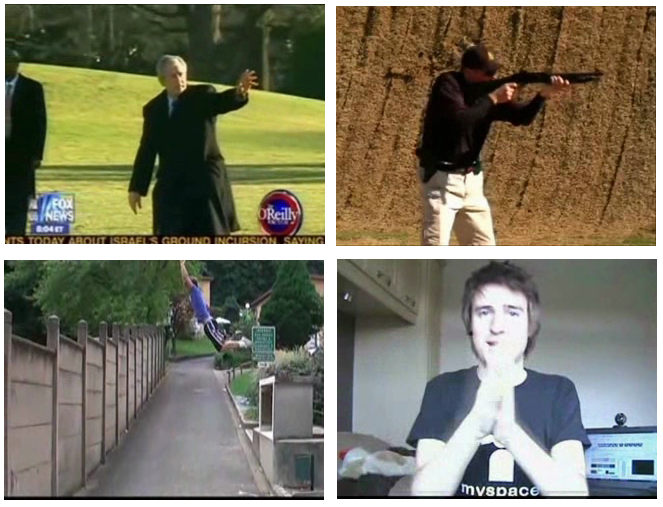
\includegraphics[width=0.7\textwidth]{jhmdb_example_images.png}
    \caption{Four example images from the JHMDB dataset \cite{jhuang_towards_2013}. }
    \label{fig:jhmdb_example_images}
\end{figure}

The puppet tool defines $15$ different joints.
They are identical to the ones annotated in the Penn Action dataset, but additionally contain \textit{neck} and \textit{belly}.
The same procedure was used to map the joints to the format provided by the MPII dataset.
Also, the approach for computing ground truth bounding boxes, as well as preprocessing the \textit{fragments} and augmentations is identical to the one presented earlier.

\section{Evaluation Metrics}
\subsection{PCK}
\label{sec:exp-pck}

The \textit{Probability of Correct Keypoints (PCK)} metric \cite{ferrari_progressive_2008} is often used in the literature to evaluate estimated pose when a human bounding box is given.
See \sref{sec:pck_related_work} for a historical motivation of this metric.
To determine if a predicted keypoint location $k_{est} = (x_{est}, y_{est})$ is estimated close enough to the ground truth keypoint $k_{gt} = (x_{gt}, y_{gt})$, first the absolute distance $d = \lVert k_{est} - k_{gt} \rVert$ is computed.
Afterwards, the maximum $l_{max} = max(bbox_{height}, bbox_{width})$ of the bounding box side lengths is computed and multiplied by a hyperparameter $\alpha$, resulting in $l_{comp} = l_{max} \cdot \alpha$.
Then, a keypoint is determined to be estimated correctly if $d < l_{comp}$.
Typical values for $\alpha$ found in the literature are $0.2$ and $0.1$.
This metric is used primarily for evaluating pose on the JHMDB dataset since it does not provide head bounding box annotations, which are necessary for using the PCKh metric.

\subsection{PCKh}
\label{sec:exp-pckh}
One downside of using the PCK metric based on person bounding box side lengths is that, for highly articulated poses, the bounding box is not always an accurate representation of the body size.
Thus, the threshold $l_{comp}$ highly depends on the pose performed.

In \cite{andriluka_2d_2014}, the authors thus propose to use the head bounding box diameter, assuming that this bounding box does not change for different poses.
See \sref{sec:pose-machine-evaluation} for a detailed historic motivation of the metric.
In most cases, $\alpha$ is set to $0.5$ and $0.2$.

\subsection{Single- and Multi-Clip Accuracy}
To evaluate the accuracy of the HAR pipeline, the authors in \cite{luvizon_2d/3d_2018} use two different approaches.
First, they take the video clip to evaluate and extract a $16$ frame fragment from the middle of the clip.
Then, they estimate the action performed.
Since the output of the network is a Softmax activation, they use the \textit{argmax} function to determine the action with the highest score.
This is referred to further as Single-Clip accuracy.

Additionally, the authors extract multiple $16$ frame fragments from the clip by starting at frame $0$ and then incrementing the starting position by $8$ for as long as there are at least $16$ frames left in the clip.
Then, for each fragment, they predict the action identical to the Single-Clip accuracy.
If the majority of the fragments estimated the same action, this is used to determine the Multi-Clip accuracy. 

\section{Experimental Results}
\subsection{Accuracy of Soft-argmax function}
For evaluating the accuracy of the Soft-argmax function, we performed two experiments.
For both experiments, an estimated coordinate $(x_{est},y_{est})$ was considered to be correct in comparison to the ground truth coordinate $(x_{gt}, y_{gt}$ if both $\lvert x_{est} - x_{gt} \rvert \leq d$ and $\lvert y_{est} - y_{gt} \rvert \leq d$, allowing for a $d$ pixel discrepancy between prediction and ground truth.
The reason for using a threshold of $d$ pixels was that the output of the Soft-argmax function are fractions of width and height with $(x_{frac}, y_{frac}) \in [0,1]$.
To compute the image coordinate, a multiplication with the width and height of the input image as well as a rounding step is necessary, possibly introducing rounding errors.

First, synthetic images of size $255 \times 255$ pixels were created, since this is the size of the input images to the network after preprocessing.
At each $x,y$ position, a two-dimensional gaussian with mean $(x,y)$ and covariance $c$ was placed.
Afterwards, the expectations were computed using the Soft-argmax function and compared to the ground truth mean value.
We chose to set $d=2$.
Performing this for each pixel coordinate and different covariances $c$, it was observed that the Soft-argmax function accurately regressed the true expectation for small covariances.
As the covariance increases, the accuracy decreases, especially around the borders.
See \fref{fig:softargmax_variance_test} for a visualization, where violett pixels indicate a wrong prediction and yellow pixels indicate a correct prediction.
As can be seen, the Soft-argmax function gets less accurate the higher the covariance is, as well as the closer the mean is to the border of the image.
This could lead to wrong estimations for training images where the joint coordinates are close to the border of the image.

\begin{figure}[htb!]
    \centering
    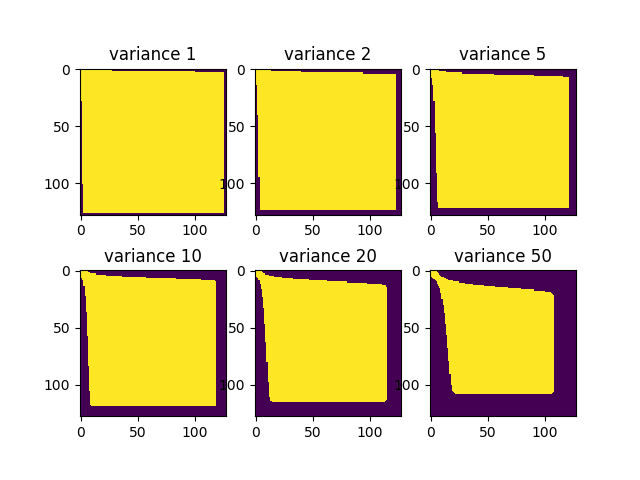
\includegraphics[width=0.7\textwidth]{softargmax_variance_test.png}
    \caption{Evaluation of the accuracy of the Soft-argmax function using synthetic data. Yellow pixels $i,j$ indicate where the Soft-argmax function correctly regressed the peak of the gaussian with mean value $i,j$, while violett indicates wrong predictions. Notice that the accuracy decreases when approaching the border of the image and when the covariance is increasing. }
    \label{fig:softargmax_variance_test}
\end{figure}

Second, to evaluate the impact of this behaviour on actual data, we analyzed the accuracy quantitatively.
Synthetic joint heatmaps were generated by placing gaussians at the position of the ground truth pose coordinates of a subset of the MPII dataset and the distance between the computed coordinates and ground truth coordinate was computed with different covariance values $c$.
We evaluated different values for $d$ and found that the the Soft-argmax function is generally accurate within a $2$ pixel window for reasonable covariance values.
The experiment was conducted on $1000$ random images from the MPII dataset.
See  for the mean accuracies achieved for covariances $c \in \{1, 2, 5, 10, 20, 50 \}$ and distances $d \in \{1, 2, 3, 4\}$.

As can be seen in \tref{tab:softargmax_numeric_eval}, the Soft-argmax function is accurate in practice for a $2$ pixer threshold.
Notice that the accuracies are significantly lower for a $1$ pixel threshold.
This contrast between $d=1$ and $d=2$ is most likely due to the rounding errors discussed earlier.

\begin{table}[]
    \centering
    \scalebox{0.90}{%
    \begin{tabular}{|l|l|l|l|l|l|l|}
    \hline
    threshold & \textbf{$c=1$} & \textbf{$c=2$} & \textbf{$c=5$} & \textbf{$c=10$} & \textbf{$c=20$} & \textbf{$c=50$} \\ \hline
    $1$ & 33.829 & 33.809 & 33.768 & 33.707 & 33.584 & 33.190 \\ \hline 
    $2$ & 99.952 & 99.931 & 99.843 & 99.741 & 99.469 & 98.598 \\ \hline 
    $3$ & 99.959 & 99.945 & 99.891 & 99.809 & 99.639 & 99.054 \\ \hline 
    $4$ & 99.959 & 99.952 & 99.911 & 99.829 & 99.700 & 99.197 \\ \hline 
    \end{tabular}}
    \caption{Mean average accuracy (in percent) of Soft-argmax when detecting ground truth coordinates from synthetic joint heatmaps. Threshold referrs to the amound of pixels the estimate is allowed to deviate from the ground truth annotation. $c$ referres to the covariance used for creating the synthetic heatmaps. The large discrepancy between a threshold of $1$ and a threshold of $2$ is most likely due to rounding errors.}
    \label{tab:softargmax_numeric_eval}
\end{table}

In summary, while the Soft-argmax function appears to be less accurate around the borders of the image, this does not effect the accuracy significantly when estimating actual pose coordinates, according to our experiments.

\subsection{Replication of Original Work}
\label{sec:exp-replication}
- first, pose estimation results on mpii were replicated
- second, 2d har on penn action is replicated

\subsubsection{Pose estimation}

- ablation study
    - vary the number of blocks
    - vary the number of context heatmaps
- explain testing procedure (also flipping)
    - explain why not all experiments can be tested
- parameters
    - learning rate 1e-3 since authors use that

\begin{figure}[htb!]
    \centering
    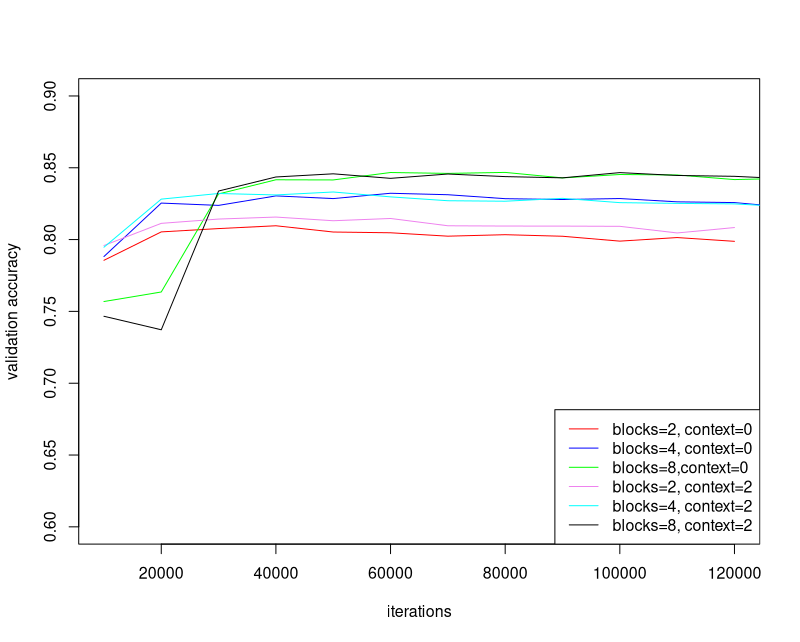
\includegraphics[width=0.7\textwidth]{mpii_vals.png}
    \caption{Validation accuracies of all evaluated pose estimation configurations on the MPII dataset. Notice that the addition of context heatmaps does not significantly improve upon the accuracy for $nr\_blocks > 2$. }
    \label{fig:mpii_vals}
\end{figure}

\begin{table}[]
    \small
    \begin{tabular}{|l|c|c|c|c|}
    \hline
        & \textbf{nr\_blocks} & \textbf{nr\_context} & \textbf{PCKh @ 0.5 (validation)} & \textbf{PCKh @ 0.5 (test)} \\ \hline
    \textbf{Own} & 2 & 0 & 80.96 &  \\
    \textbf{} & 2 & 2 & 81.56 &  \\
    \textbf{} & 4 & 0 & 83.22 &  \\
    \textbf{} & 4 & 2 & 82.97 &  \\
    \textbf{} & 8 & 0 & 84.67 &  \\
    \textbf{} & 8 & 2 & 84.66 & tbd \\ \hline
    \textbf{\cite{luvizon_2d/3d_2018}} & 8 & 2 & 89.00 & 91.2 \\ \hline
    \end{tabular}
\end{table}

\begin{table}[]
    \centering
    \scalebox{0.90}{%
    \begin{tabular}{|l|l|l|l|l|l|l|l|l|}
        \hline
        &Head & Shoulder & Elbow & Wrist & Hip & Knee  & Ankle & Total  \\ \hline
        out recreation& 95.7  & 90.5  & 81.4  & 74.6  & 82.5  & 73.0 & 66.2 & 81.4 \\
        \cite{luvizon_2d/3d_2018}& 98.1  & 96.6  & 92.0  & 87.5  & 90.6  & 88.0 & 82.7 & 91.2  \\ \hline
    \end{tabular}}
    \caption{Our recreation in direct comparison to the original work by \cite{luvizon_2d/3d_2018}. Values represent PCKh using $\alpha = 0.5$.  } %TODO: New values and / or explain differences
    \label{tab:softargmax_numeric_eval}
\end{table}

\subsubsection{HAR using Penn Action dataset}

- train pose estimator using 75 mpii 25 penn action, as did the authors
- parameters
    - augmentation of 75 augmented and 25 regular (for all experiments, if not mentioned otherwise)
    - batch size 30
    - learning rate 1e-3 because thats what the authors use in their MPII training. they do not talk about the learning rate used for this
    - trained for 110000 iterations (batches)
- PCK @ 0.2 used for evaluation 
% TODO: Test using PCK @ 0.2 and @ 0.1
% TODO: statistical significance testing
% TODO: discuss gt_bb 

- first find the point where validation plateaus
- parameters
    - batch size 12
    - for X iterations, afterwards validation plateaus % TODO
    - learning rate 2e-5 since this is what the authors used
    - 4 blocks, 2 context in pose estimation

- Started finetuning at iteration X and reduce learning rate by X % TODO
- Talk about results
% TODO: statistical significance testing

\subsection{Pose estimation on JHMDB dataset}

- same ablation study as before
    - evaluate different number of blocks and context heatmaps
        - talk about a general conclusion like \textit{the higher the number of blocks the better}
- parameters
    - learning rate 1e-3, as discussed in MPII

% TODO: report the number of iterations used
% TODO: do plot of all validation accuracy cuvers
- general conclusion: is this dataset harder? why?

\subsection{HAR on JHMDB Dataset}
%all kinds of substitutions like using gt bb etc.
- use the pretrained pose estimator from before, 4 blocks, 2 context heatmaps
- parameters
- Same as in pennaciton: first find the validation plateau point
- afterwards: new experiment with finetune

\subsection{Effect of Combining Loss Functions}
- explain how e2e training was done (using pose loss etc.)
- show results
- explain why it didnt work (or why it did)

\subsection{Effect of Using Different Representations of Pose}
\label{sec:different_pose_representation_experiment}

